\title{Singularity Software\\Milestone 5}
\date{\today}

\documentclass[12pt]{article}
\usepackage[a4paper]{geometry}
\usepackage{makeidx}
\usepackage[acronym]{glossaries}
\usepackage{lscape}
\usepackage{amsmath}
\usepackage{graphicx}
\usepackage[final]{pdfpages}
% \usepackage{hyperref} % Makes links from ToC

\geometry{top=1.0in, bottom=1.0in, left=1.0in, right=1.0in} % Sets the margins

\setlength{\parindent}{0pt} % Fixes the paragraph spacing problem

% This is all for formatting and making the Table of Contents according to 
% spec. Don't play with it.
\makeatletter
\renewcommand\l@section[2]{%
  \ifnum \c@tocdepth >\z@
    \addpenalty\@secpenalty
    \addvspace{1.0em \@plus\p@}%
    \setlength\@tempdima{1.5em}%
    \begingroup
      \parindent \z@ \rightskip \@pnumwidth
      \parfillskip -\@pnumwidth
      \leavevmode \bfseries
      \advance\leftskip\@tempdima
      \hskip -\leftskip
      #1\nobreak\ 
      \leaders\hbox{$\m@th\mkern \@dotsep mu\hbox{.}\mkern \@dotsep mu$}
     \hfil \nobreak\hb@xt@\@pnumwidth{\hss #2}\par
    \endgroup
  \fi}
\makeatother

\makeindex

% Construct the glossary here
% Use the template below, then where the word appears (in the case below, computer), replace computer with \gls{computer}
\makeglossaries

\newglossaryentry{Sifteo Cubes}
{
  name={Sifteo Cubes},
  description={are small machines capable of loading programs and interacting with one another as well as responding to predefined movements}
}

\newglossaryentry{Object-Oriented Programming}
{
  name={Object-Oriented Programming},
  description={is a programming paradigm using objects to design applications}
}

\newglossaryentry{Windows}
{
  name={Windows},
  description={is a series of operating systems developed by Microsoft}
}

\newglossaryentry{Mac}
{
  name={Mac},
  description={is a series of lines of personal computers developed by Apple}
}

\newglossaryentry{Linux}
{
  name={Linux},
  description={is a Unix-based operating system based on free and open source software}
}

\newglossaryentry{cross-platform support}
{
  name={cross-platform support},
  description={is an attribute given to software implemented and operable on multiple computer platforms}
}

\newacronym{API}{API}{\glsadd{API}{Application Programming Interface}}

\newglossaryentry{APIg}
{
  name={Application Programming Interface},
  description={is an interface implemented by a software program that enables it to interact with other software}
}


\newglossaryentry{open source}
{
  name={open source},
  description={is an attribute given to software for which the source code is freely available}
}

\newacronym{IDE}{IDE}{\glsadd{IDE}{Integrated Development Environment}}

\newacronym{SDK}{SDK}{\glsadd{SDK}{Software Development Kit}}

\newglossaryentry{SDKa}
{
  name={Software Development Kit},
  description={is a collection of tools designed to help build software for a particular platform. It may include an \index{API} and an emulator of the target platform among other things.}
}

\newglossaryentry{IDEa}
{
  name={Integrated Development Environment},
  description={is software that provides a comprehensive work environment for computer programmers and software developers}
}


\newacronym{GUI}{GUI}{\glsadd{GUI}{Graphical User Interface}}

\newglossaryentry{GUIa}
{
  name={Graphical User Interface},
  description={is a visual way of allowing the user to interace with a computer program}
}

\newglossaryentry{version control}
{
  name={version control},
  description={is the management of documents and programs for a project over many versions in a well-organized manner}
}

\newglossaryentry{issue tracking system}
{
  name={issue tracking system},
  description={is a piece of software used to maintain a list of issues as generated during a project}
}

\newglossaryentry{usability study}
{
  name={usability study},
  description={is a manner of evaluating the design and user experience of a product by testing it on users}
}

\renewcommand*\arraystretch{1.5}

\begin{document}
\vspace*{\fill}
        \begin{center}
                \LARGE{Singularity Software} \\
                \LARGE{\textit{Milestone 5}} \\
                \vspace{.15in}
                \large{\today} \\
                \vspace{4in}
                By signing below, I approve the contents of the following document. \\
                \begin{table}[h]
                        \begin{tabular}{p{2in} p{5.5in}}
%                \begin{align*}
                        & \\
                        Alex Mullans & \line(1,0){285} \\ & \\
                        Ruben Rodriguez & \line(1,0){285} \\ & \\
                        Ethan Veatch & \line(1,0){285} \\ & \\
                        Kurtis Zimmerman & \line(1,0){285}
                        \end{tabular}
                \end{table}
%                \end{align*}
        \end{center}
\vspace*{\fill}
\thispagestyle{empty}

\clearpage

\tableofcontents

\clearpage
        
\section{Executive Summary}
This document is the fifth and final in a series of milestone documents that will accompany the planning of the Siftables\index{Siftables} Emulator\index{emulator}. The Emulator project is an application that will allow developers of Sifteo applications to test the features of Sifteo Cubes --- miniature computers that interact and communicate when used in tandem --- in a virtual programming environment. There is currently an emulator from Sifteo, Inc. that comes as part of the \gls{SDK}\index{SDK}\glsadd{SDKa} for the Cubes. However, Singularity intends to come up with a more natural interface than the one currently provided in that application.\\\\
This milestone reports on the usability study that was conducted to compare the interfaces of Sifteo Inc.'s Siftulator and Singularity's Siftables Emulator. After elaborating the methods and findings of that study, it goes on to show the original prototype used therein as well as a second prototype that has been adjusted based on feedback therefrom.

\section{Introduction}
Developers of applications for the \gls{Sifteo Cubes}\index{Sifteo} currently must test programs they create for the platform within the emulator provided by Sifteo. While this emulator covers all  the functionality of the Sifteo Cubes, it presents a user interface that Singularity Software believes could be more naturally implemented. As such, Singularity Software will provide, in the form of the Siftables Emulator\index{emulator}, a new software-based emulator\index{emulator} for the Sifteo Cubes that will allow developers to more naturally interact with the platform.\\\\
Milestone 5 elaborates on the \gls{usability study} that compared the proposed Siftables Emulator design to the Siftulator's design before presenting original and feedback-based interface designs for the Siftables\index{Siftables} Emulator\index{emulator}. It follows Milestones 2, 3, and 4, which defined a change control plan, coding standards, test cases, and requirements of the Siftables Emulator specification based on the high-level design created in Milestone 1. 

\section{Project Background}
The Siftables Emulator is being developed by Singularity Software as part of the Junior Project sequence of classes at Rose-Hulman Institute of Technology. When projects were solicited for the sequence, clients Tim Ekl and Eric Stokes (both Rose-Hulman alumni) submitted a request for an emulator\index{emulator} for Sifteo Cubes, a new platform intended for ``intelligent play." After Singularity was chosen for the project, we met with Mr. Ekl to determine the three primary features of the Emulator: a Workspace where 1-6 Cubes could mimic the manipulations possible with physical Cubes, an \gls{API} to program those virtual Cubes, and a set of example games designed to show off the first two features. Singularity's Emulator\index{emulator} is intended to build on the foundation of Sifteo, Inc.'s existing emulator by creating a more fluid and natural user interface.

\section{Usability Report}

\subsection{Process}
In order to conduct the usability test, a basic prototype of the Siftables Emulator was developed using Adobe Flash CS5. The prototype, which modeled the basic functionality intended for the final emulator, was then compared to the current Sifteo Inc. emulator, the Siftulator. The tests were conducted using CSSE students and faculty as subjects, because the primary target demographic of the software is developers. \\\\
Participants in the study were first presented with an informed consent form and a pre-test questionnaire that collected relevant personal information. Upon completion of these two documents, the user was then taken into the testing area and given a brief set of verbal instructions by one of the team members. After the team member finished presenting the instructions and left the room, the participant was asked to begin the study by watching a short video demonstrating the capabilities of the Sifteo Cubes. We felt that this was the most efficient way to acquaint users with the product and we believed that it was necessary for them to be able to accurately judge the performance of an emulator. \\\\
Upon completion of the video, participants were asked to complete a series of simple tasks in the current Siftulator platform. Because of the nature of this product and its lack of a help file, a list of action commands from Sifteo's website was located on the table next to the user. If they could not intuitively determine the correct way to complete a task, participants were told that this sheet could be used to help them. Users were then asked to switch to Siftables Emulator prototype and reminded that this product was in no way based on the software which they had just used. They were then asked to complete a similar set of tasks using the prototype. In the event that the user became stuck and was unable to complete their task at any time on either emulator, help was offered. This help was kept to a minimum, often consisting solely of asking the user a question to help them cogitate in a different fashion. \\\\
At the conclusion of the technical portion of the study, participants were thanked for their time and assistance and asked to complete a post-test questionnaire. This questionnaire was designed to allow each user to express his or her opinion about the various aspects of both projects and suggest possible improvements to the interface of the Siftables Emulator prototype.

\subsection{Analysis}
The results from the usability study can be found primarily in the usability report generated by the Ovo software. \\\\
Additionally, a pre-test questionnaire and a post-test questionnaire were distributed to each participant to collect data regarding their overall experience as well as their prior knowledge of the product and similar systems. The informed consent form, pre-test questionnaire, and post-test questionnaire are all included as appendices at the end of this document. The results of the questionnaires are shown in the table following this section.

\subsubsection{Pre-Test Results}
\begin{enumerate}
        \item{All of the participants reported that they had never heard of Sifteo nor their product. This lack of previous experience working with the product provided a clean slate on which to base our findings.}
        \item{All of the participants but one reported having never programmed for an embedded system before. This question does not directly reflect in any of the results, but it indicates that the emulator is still accessible to first-time programmers for embedded systems.}
        \item{On average the participants felt somewhere between comfortable and uncomfortable using new software without documentation.  As  that is the exact median of the possible values, these results are expected.}
        \item{With documentation, all participants felt at least somewhat comfortable, and all but one reported feeling very comfortable using new software. Because the participants chosen were all from or had experience in the field of computer science/engineering or software engineering, this is expected.}
        \item{Similar results were found with the participants' comfort level with using an API.}
        \item{Half of the participants had used an emulator before, and half had not, indicating that our results would accurately depict the user experience on both ends of the spectrum.}
\end{enumerate}

\subsubsection{Study Results}
Results from the usability study with the six participants are available in the usability report. Overall, the times associated with the tasks for Singularity's emulaor were significantly lower than those associated with the tasks for Sifteo's emulator.  \\\\
One notable difference was in the ``Load program'' task.  Using Sifteo's emulator, a user has to open a separate program loader, and navigating to the ``Play'' functionality is not intuitive.  Additionally, there is not much immediate feedback regarding the success of loading a program.  On the other hand, in Singularity's emulator, loading a program was literally as easy as the click of a button, making the task much more straightforward.

\subsubsection{Post-Test Results}
\begin{enumerate}
        \item{All but one participant strongly agreed that the main screen of the emulator was accessible. The other participant agreed that the main screen was accessible but did not strongly agree, indicating that the layout works well for efficient use.}
        \item{All but two participants strongly agreed, and the other two agreed, that the commands were in easy-to-find locations, reinforcing that the layout of the main screen was well-designed.}
        \item{Moving a Cube was not as straightforward; on average, users agreed that it was easy, but one participant strongly disagreed.  Because the moving functionality was not fully implemented in the prototype but participants found it easy to use in Sifteo's emulator, we can ensure that the functionality will be easy to use because we plan on implementing movement in the same way.}
        \item{Organizing Cubes on the screen on average was determined to be halfway between agreeing and strongly agreeing. Because only one Cube was present in the emulator, some found it less intuitive because they did not receive visual feedback, which is understandable and does not heavily indicate any lack of usability in the product.}
        \item{Manipulating a Cube on average was indicated to be fairly intuitive, but not all functionality was straightforward or immediately obvious.  As the study indicated, shaking and tilting took considerably longer than the other manipulations; some users found the icons associated with these movements unintuitive.}
        \item{On average, the participants agreed that Singularity's emulator was easier to use than Sifteo's.  The participants who found Sifteo's emulator easier to use made extensive use of the help sheet provided, so they were able to complete the actions more quickly.}
\end{enumerate}

\begin{landscape}
\begin{center}
  \begin{tabular}{| l | l | l | l | l | l | l | l | l | l | l | l | l | l | l |}
    \hline

    \textbf{Gender} &
    \textbf{Major} &
    \textbf{Class} &
    \textbf{Pre1} &
    \textbf{Pre2} &
    \textbf{Pre3} &
    \textbf{Pre4} &
    \textbf{Pre5} &
    \textbf{Pre6} &
    \textbf{Post1} &
    \textbf{Post2} &
    \textbf{Post3} &
    \textbf{Post4} &
    \textbf{Post5} &
    \textbf{Post6} \\ \hline

    F &
    CS &
    S &
    A &
    No &
    1 &
    4 &
    4 &
    No &
    4 &
    4 &
    1 &
    2 &
    3 &
    3 \\ \hline

    F &
    CE &
    F &
    A &
    No &
    1 &
    3 &
    4 &
    Yes &
    3 &
    4 &
    3 &
    4 &
    3 &
    4 \\ \hline

    M &
    SE/CS/MA &
    S &
    A &
    No &
    3 &
    4 &
    3 &
    Yes &
    4 &
    4 &
    4 &
    4 &
    3 &
    2 \\ \hline

    M &
    SE &
    J &
    A &
    No &
    4 &
    4 &
    4 &
    Yes &
    4 &
    3 &
    4 &
    4 &
    4 &
    2 \\ \hline

    M &
    CSSE &
    Fac &
    A &
    No &
    3 &
    4 &
    4 &
    No &
    4 &
    3 &
    2.5 &
    2.5 &
    3 &
    4 \\ \hline

    M &
    CPE &
    J &
    A &
    Yes &
    3 &
    4 &
    4 &
    No &
    4 &
    4 &
    4 &
    4 &
    4 &
    4 \\ \hline

    & & & & & & & & & & & & & & \\ \hline

    \textbf{Average} &
    & & & &
    2.5 &
    3.8 &
    3.8 &
    &
    3.8 &
    3.7 &
    3.1 &
    3.4 &
    3.3 &
    3.2 \\ \hline

    
  \end{tabular}
\end{center}
\end{landscape}

\subsection{Findings}
Based on the post-test results, our emulator was regarded as having an accessible layout and fairly intuitive controls.  All the users at least agreed that the commands were in easy-to-find locations and that the main screen looked accessible. \\\\
One aspect that the users saw could be improved is manipulating the Cube.  While rotating and flipping were not an issue for most users, they found tilting and shaking to be more difficult to comprehend.  For this reason, we made the edges of the Cube bolder to help inform the user where to grab the Cube for tilting and also changed the shake icon to be more recognizable.  However, since most of the users’ first instinct to shake the Cube was to drag it with the mouse, the shake icon is temporary and we plan to implement mouse control for the shake command in the future. \\\\
Users, on average, completed the designated tasks quicker and with less help in comparison to Sifteo’s emulator.  Overall, the emulator was viewed as an improvement over Sifteo’s emulator by outperforming it in various tasks such as adding/removing Cubes, loading programs, and controlling the Cubes.

\section{Interaction Architecture}
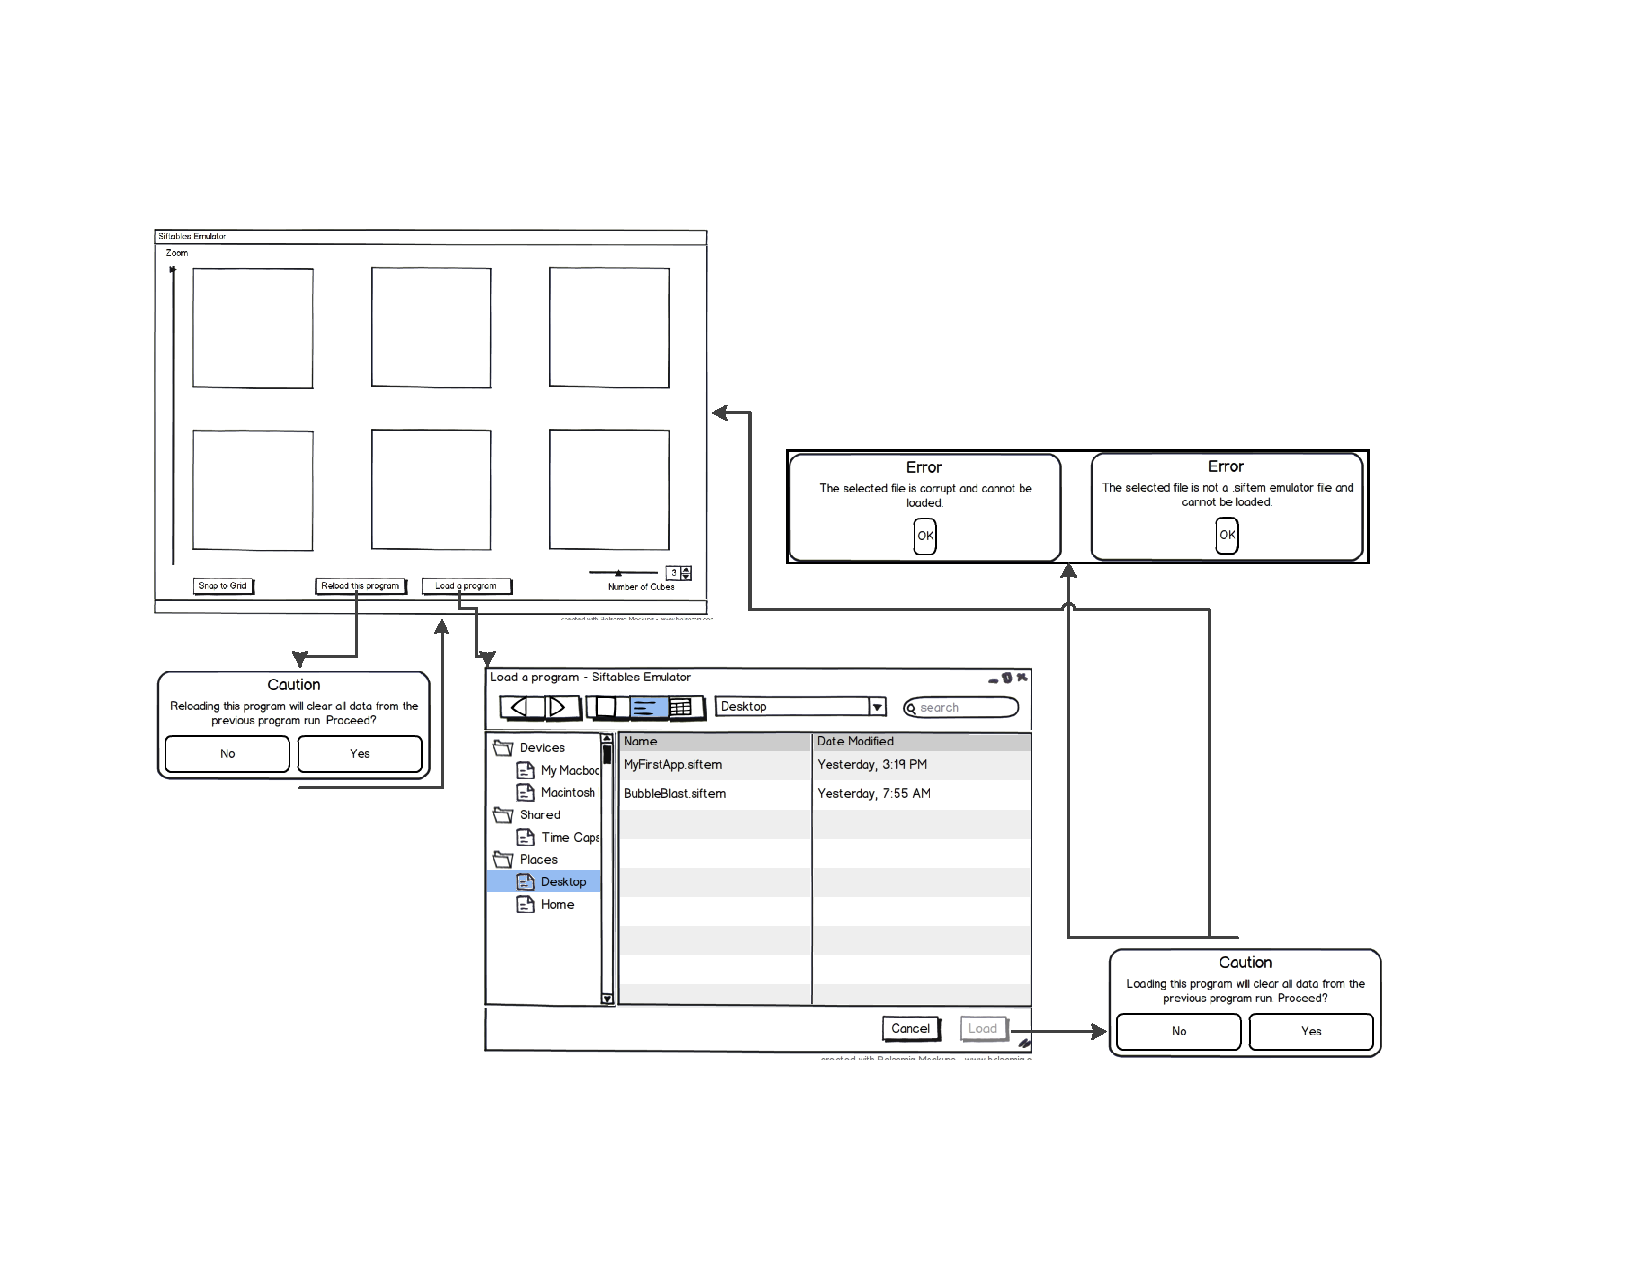
\includepdf[landscape]{interaction.pdf}

\section{Initial Interface Design}
\begin{center}
  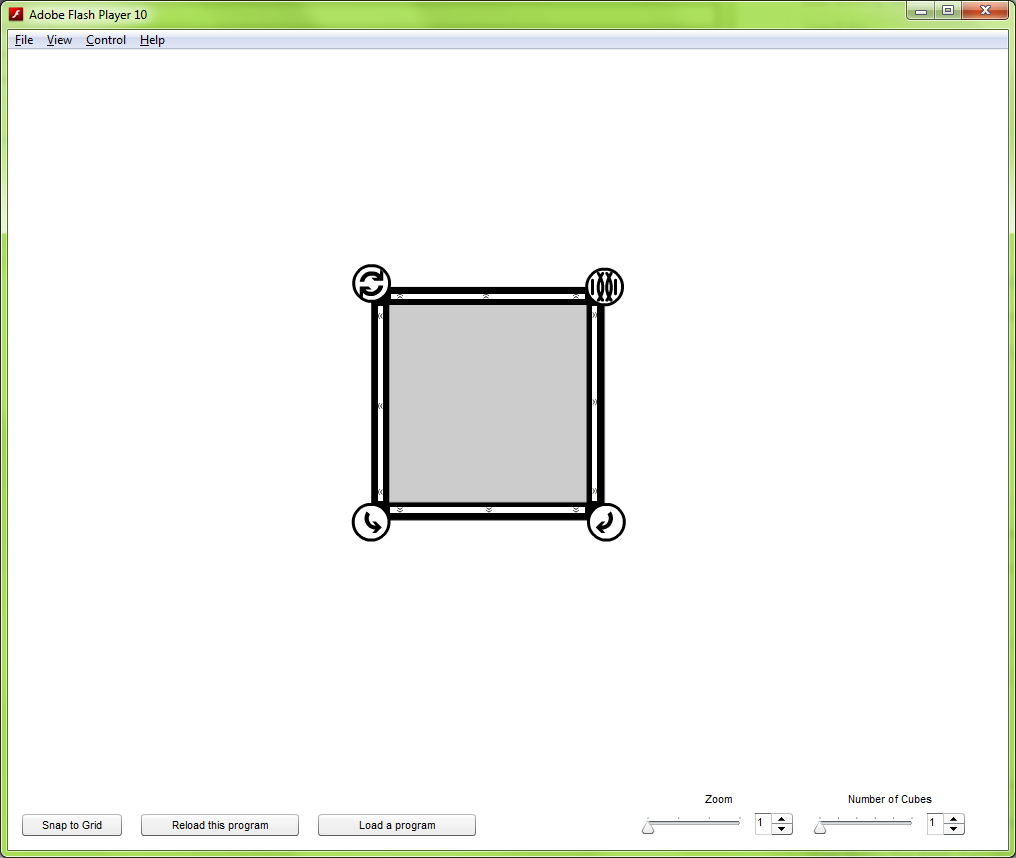
\includegraphics[scale=.4]{../prototype/prototype1.png}
\end{center}

Singularity's initial interface design was well-received. Usability testers were able to easily access all presented functions except tilt and shake.

\section{Revised Interface Design}
\begin{center}
  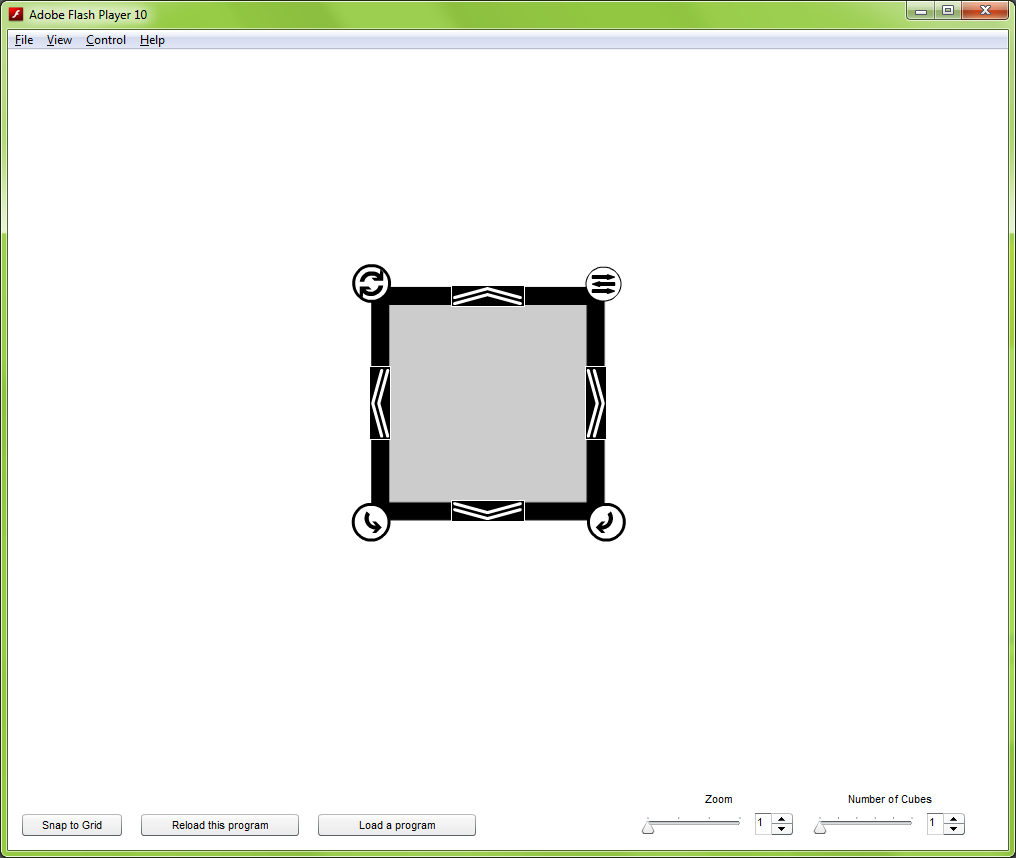
\includegraphics[scale=.4]{../prototype/prototype2.png}
\end{center}

Based on the results of the usability test, Singularity redesigned parts of the interface to make the tilt and shake actions more obvious. Specifically, we replaced the tilt buttons on each side of the cube with larger, clearer instances. Additionally, we redesigned the shake button to increase its clarity and better relate the icon to the button's purpose.

\appendix
    \begin{landscape}
    \section{Features}
    \begin{table}[h!]
      \begin{tabular}{p{1.5in} | p{2.25in} | p{.75in} | p{.75in} | p{.75in} | p{2.25in}}
        \textbf{Feature} &
        \textbf{Description} &
        \textbf{Status} &
        \textbf{Priority} &
        \textbf{Risk} &
        %\textbf{Stability} &
        \textbf{Reason} \\ \hline
        %\textbf{Effort} \\ \hline

        Individual, virtual Sifteo Cube &
        A virtual representation of a single Sifteo Cube &
        Approved &
        Critical &
        Low &
        %High &
        Replicates physical Sifteo Cube \\ \hline
        %Medium \\ \hline

        Buttons to manipulate each virtual Cube &
        Buttons on the virtual Cube will allow the user to flip and tilt it &
        Approved &
        Critical &
        Medium &
        %High &
        Replaces physical actions where said actions would be impractical with a mouse \\ \hline
        %Medium \\ \hline

        Workspace where multiple Cubes can be emulated &
        Multiple Cubes will be displayed on a workspace that replicates the free-form nature of physical Sifteo Cubes\index{Sifteo Cubes} &
        Approved &
        Critical &
        Low &
        %High &
        Replicates multiple Sifteo Cubes\index{Sifteo Cubes} in a natural, free-form environment \\ \hline
        %High \\ \hline

        Interactions between Cubes &
        The Cubes present on the workspace will communicate when they are neighbored &
        Approved &
        Critical &
        Low &
        %High &
        Cubes can simulate the interactions possible with physical Cubes \\ \hline
        %High \\ \hline

        Load programs into the Cubes &
        The user will load his own and example programs into the emulator’s\index{emulator} Cubes &
        Approved &
        Critical &
        Medium &
        %High &
        The ability to program programs for the emulator\index{emulator} is dependent on a common interface \\ \hline
        %High \\ \hline

        Snap Cubes to invisible grid &
        The Cubes will snap into an invisible grid when a button is clicked &
        Proposed &
        Useful &
        Medium &
        %High &
        Increases productivity by allowing a quick reset if the Cubes are in disarray \\ \hline
        %Low \\ \hline

        Zoom Workspace &
        The Workspace will zoom to the level of an individual Cube or the whole space &
        Proposed &
        Useful &
        Low &
        %High &
        Inspecting individual Cubes allows for precise checks of program \glspl{GUI}\index{GUI}\glsadd{GUIa} \\ \hline
        %Low \\ \hline

      \end{tabular}
    \end{table}
    \end{landscape}

    \clearpage

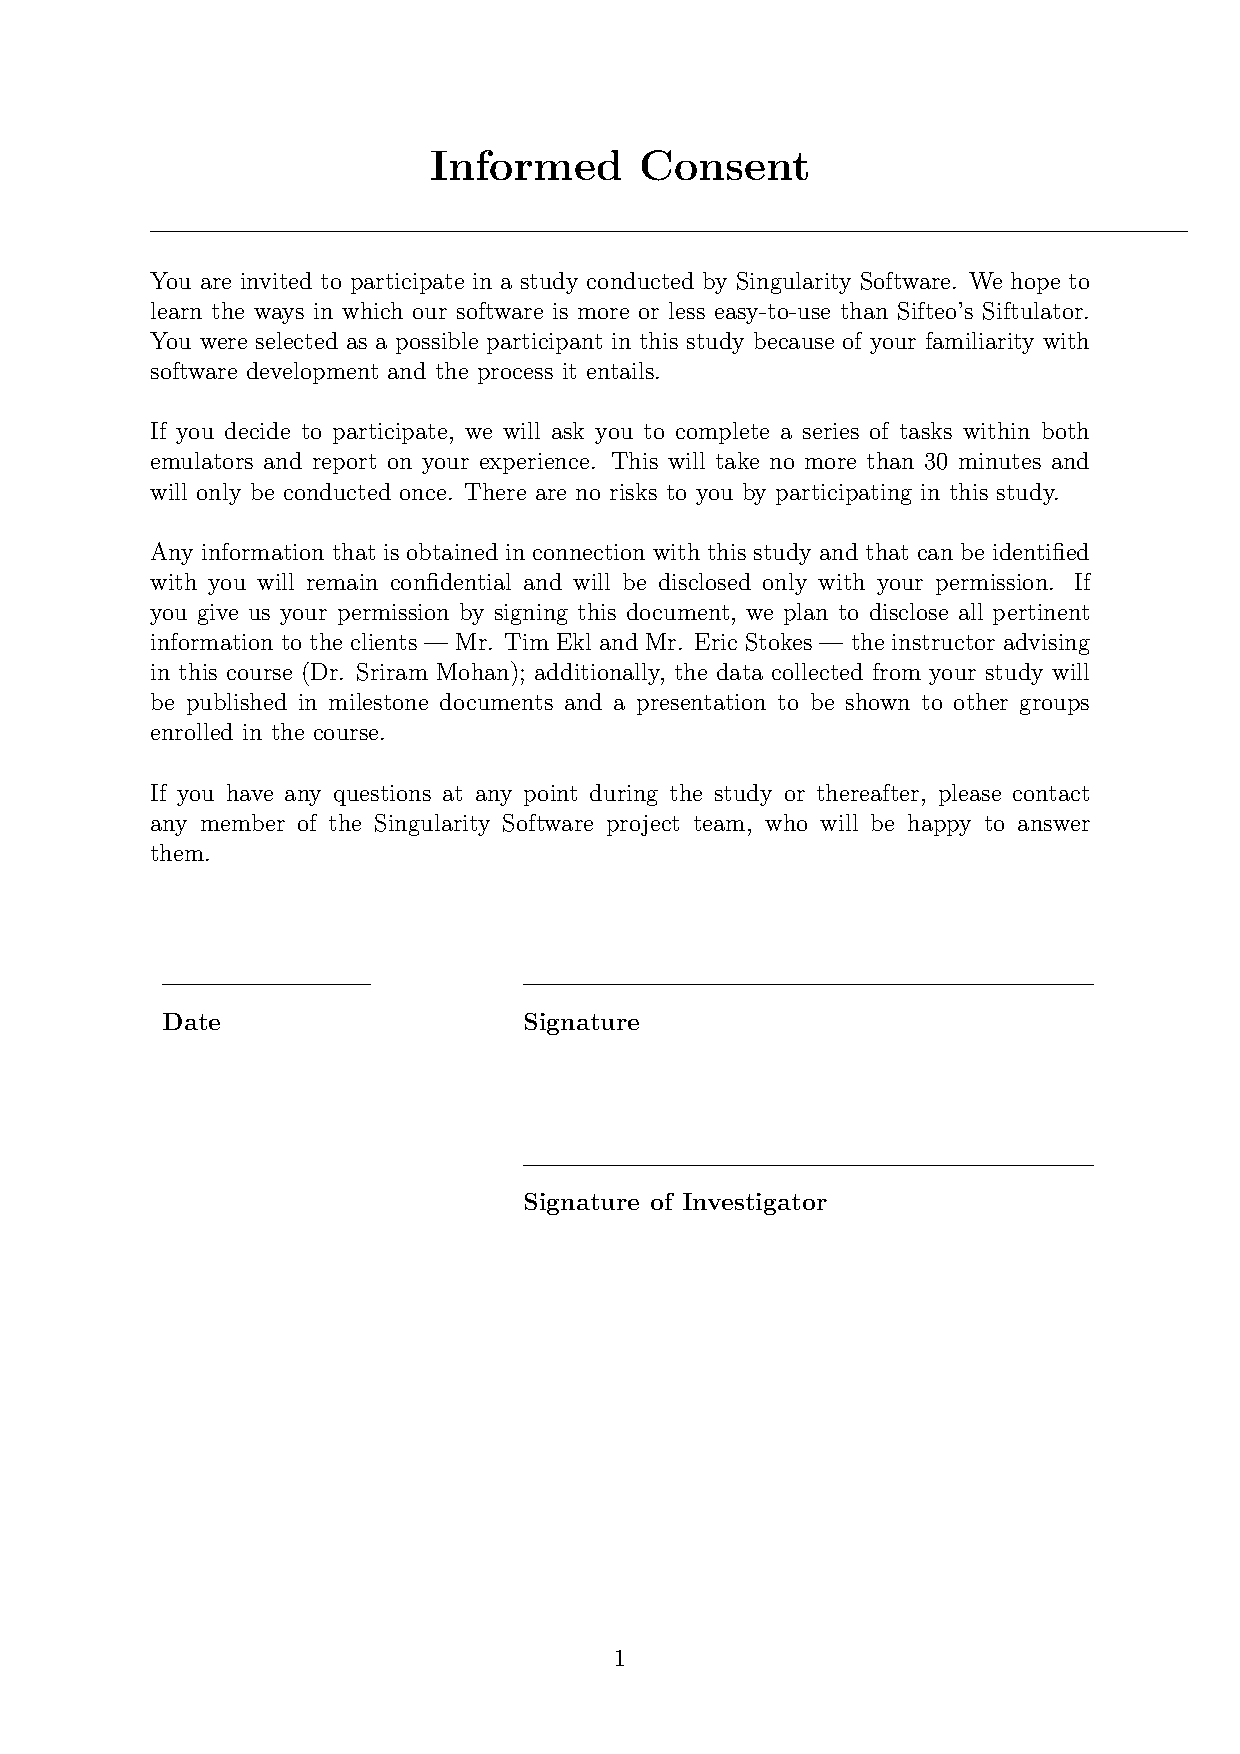
\includepdf{usability/informedConsent.pdf}
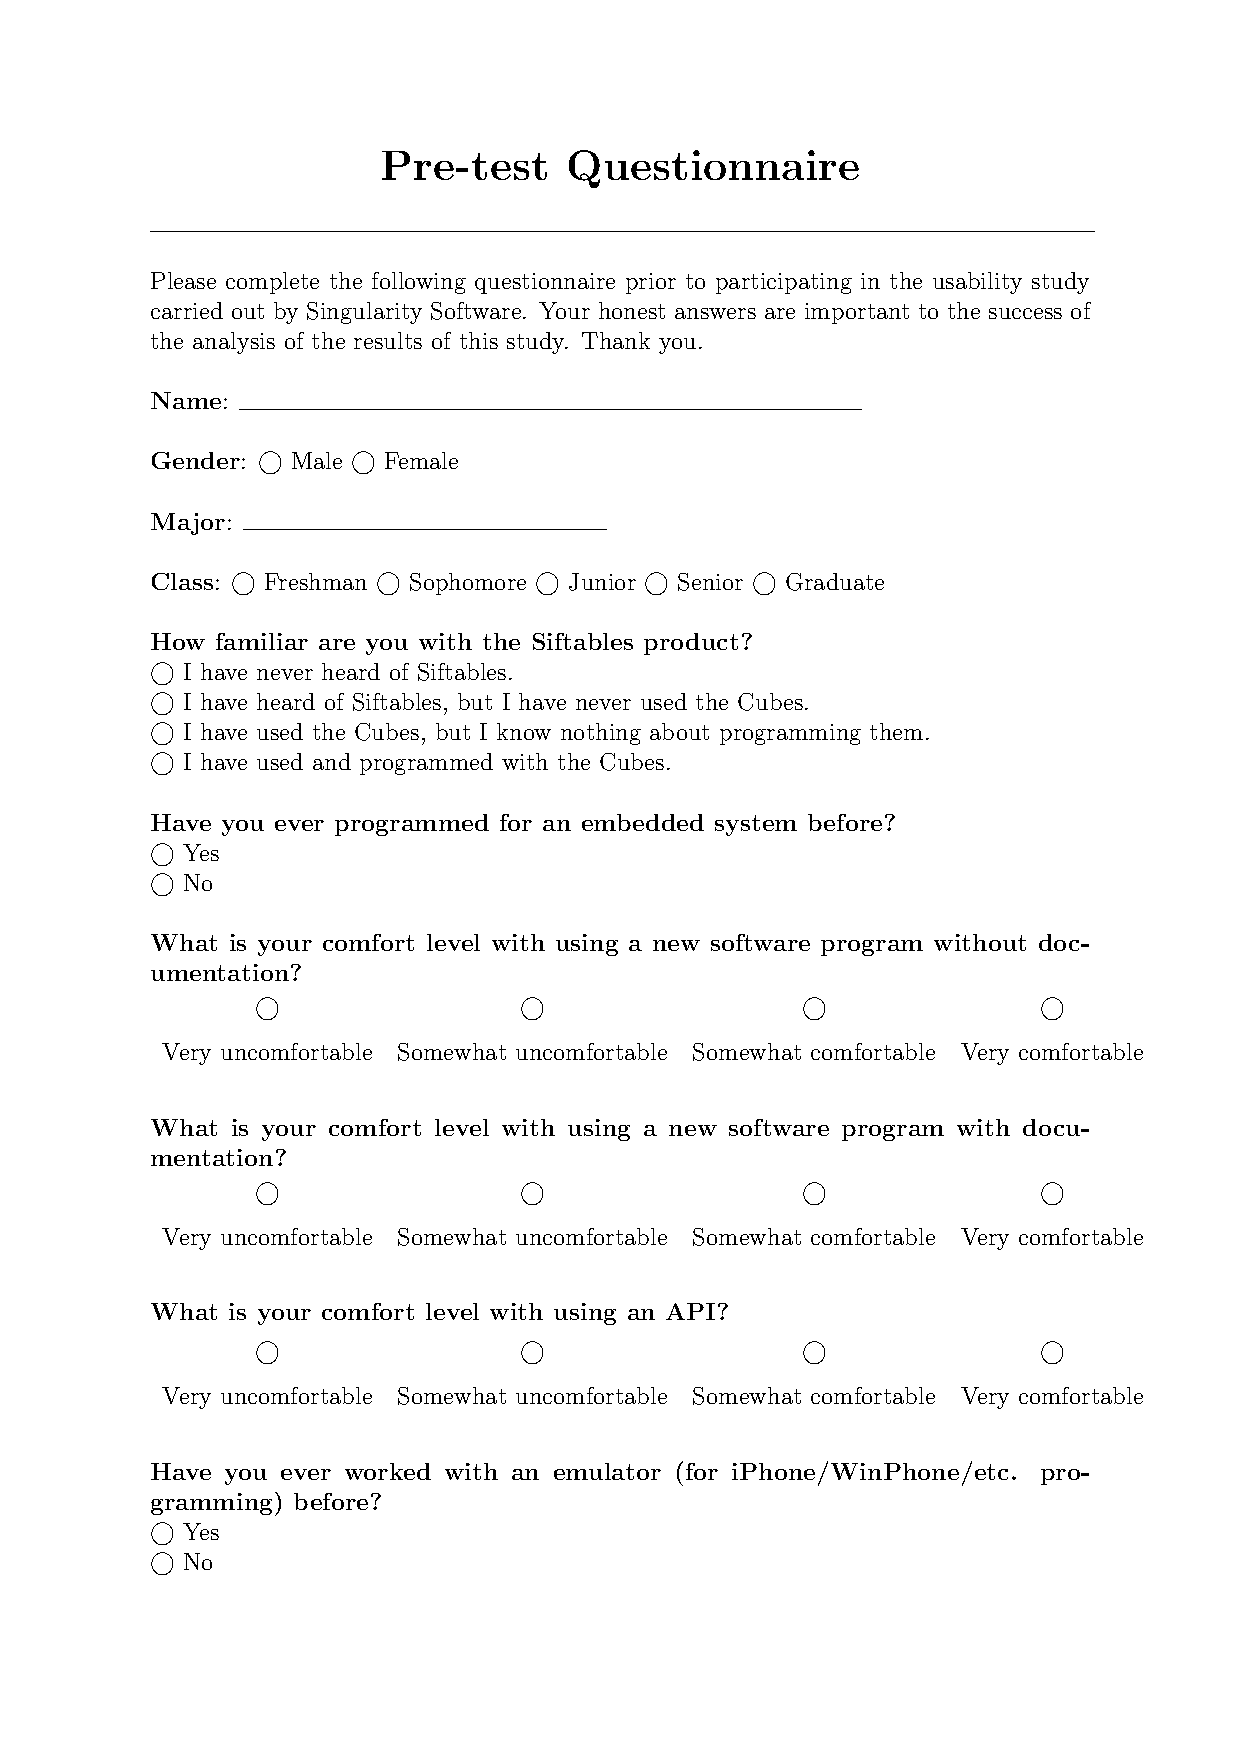
\includepdf{usability/pretest.pdf}
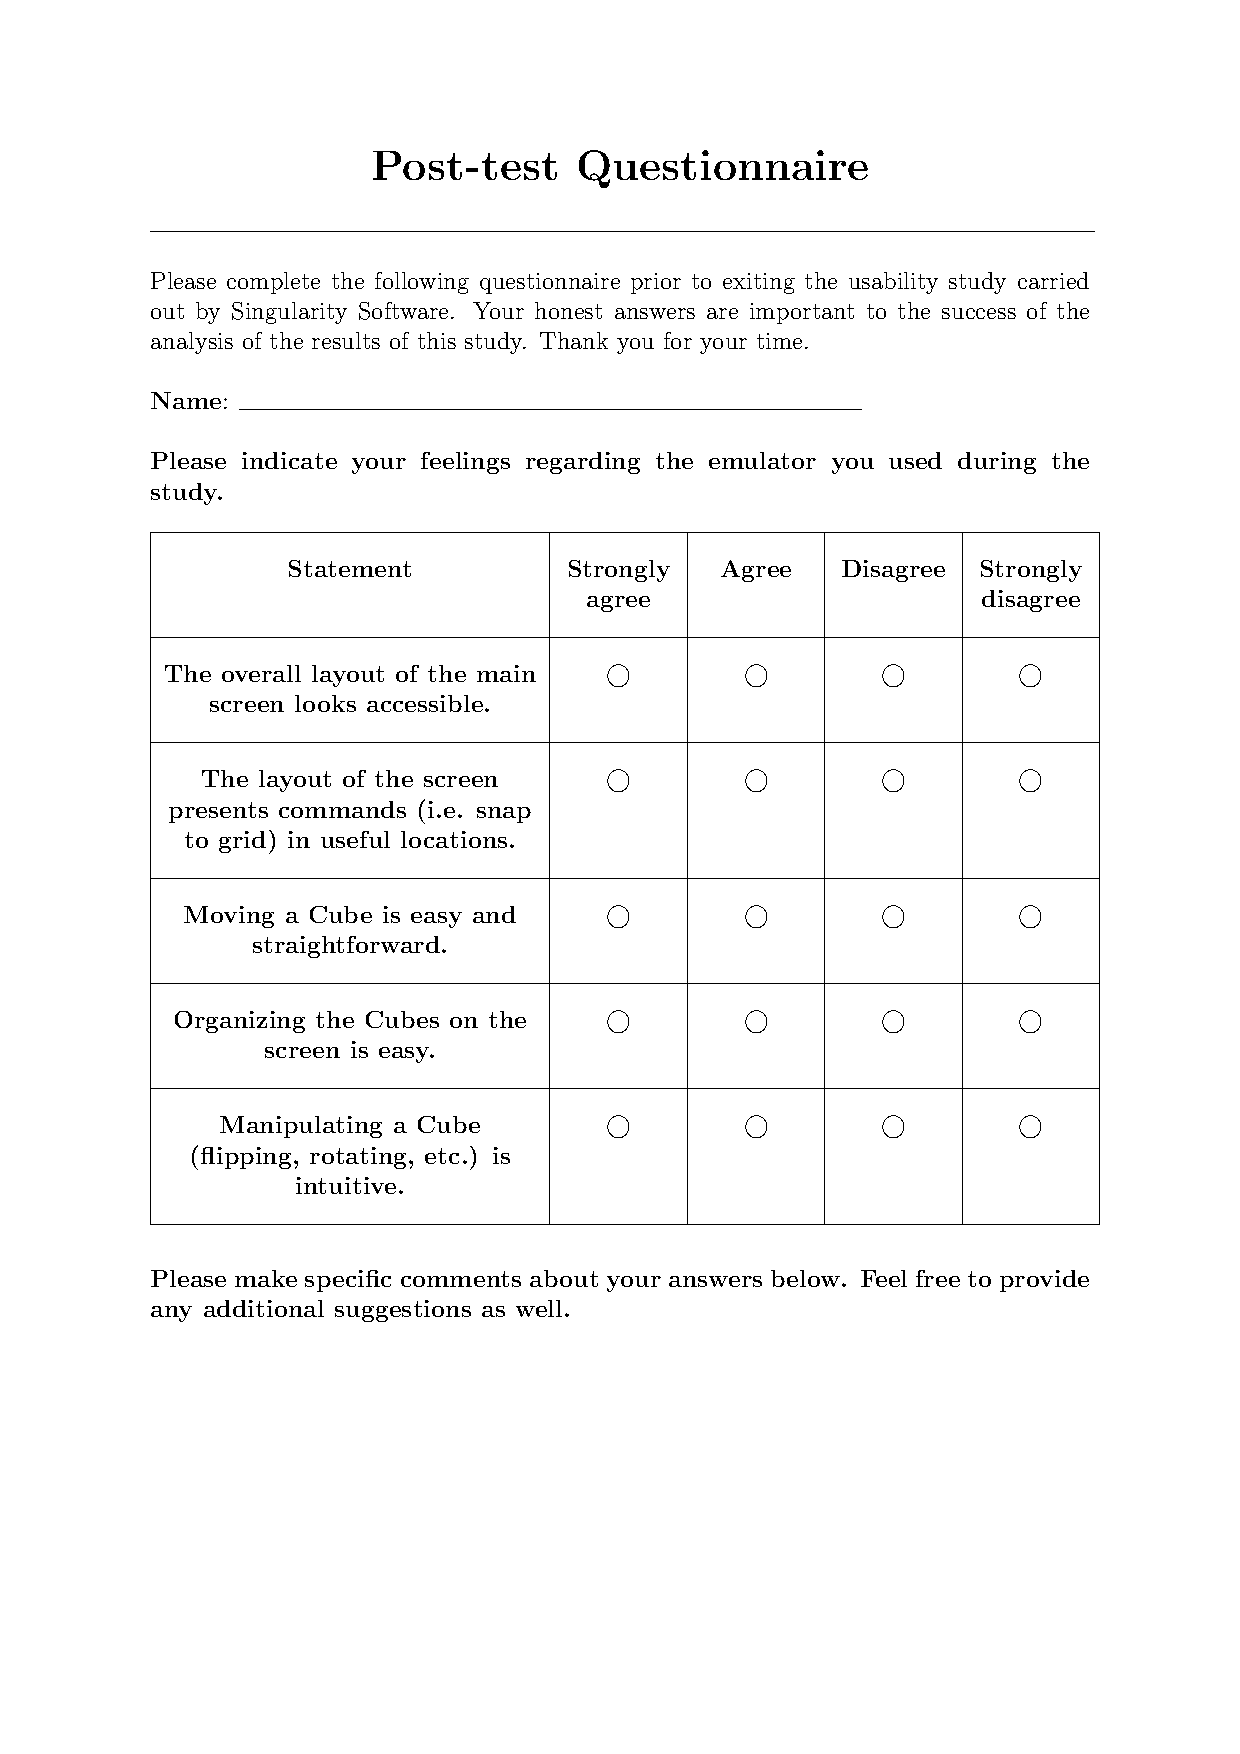
\includepdf{usability/posttest.pdf}

\clearpage
\addcontentsline{toc}{section}{Glossary}
\printglossaries
\clearpage

\addcontentsline{toc}{section}{References}
\section*{References}

        \begin{enumerate}
                \item{Sifteo Inc. Online: http://www.sifteo.com}
                \item{Tim Ekl.  Client Meeting. 25 October 2011 2:30 p.m.}
                \item{Milestone 1.  Singularity Software.  Online: https://github.com/alexmullans/Siftables-Emulator/blob/master/docs/pdfs/m1.pdf}
                \item{Milestone 2.  Singularity Software.  Online: https://github.com/alexmullans/Siftables-Emulator/blob/master/docs/pdfs/m2.pdf}
                \item{Milestone 3.  Singularity Software.  Online: https://github.com/alexmullans/Siftables-Emulator/blob/master/docs/pdfs/m3.pdf}
                \item{Milestone 4.  Singularity Software.  Online: https://github.com/alexmullans/Siftables-Emulator/blob/master/docs/pdfs/m4.pdf}

        \end{enumerate}

\clearpage

\addcontentsline{toc}{section}{Index}
\printindex

\end{document}
